

\partabstractfp{本章讲述如何根据不同类型的进程分配不同策略的调度算法,调度算法的原理及应用对象,如何更改进程的调度策略。
}
\partabstractrp{练习题:\\
\small{1. 运行2个高CPU利用率进程,调整他们的nice。\\2. 用chrt把一个死循环进程调整为SCHED\_FIFO。\\3. 阅读ARM的big.LITTLE架构资料,\\并论述为什么ARM要这么做。}}
\partabstractlettrine{L}{inux进程的类型不同,策略不同。} % the first word of the abstract

\part{进程课第3天}


\chapter{进程分类}


\section{CPU消耗与IO消耗型}
CPU消耗型是指CPU占用率高的应用,比如编译代码。IO消耗型指像读硬盘之类的应用,大部分时间消耗在DMA上,CPU占用率比较低。典型的操作系统内,IO消耗型的优先级比较高。因为IO消耗型应用往往与用户体验密切相关,比如读写硬盘和外设之类的操作,用户操作键盘和鼠标时如果长时间没有反应,就会导致体验很差。而CPU消耗型,比如编译程序,我们可以把它的优先级降低,编译时间从10分钟变成11分钟,对用户的体验影响不是很大。

IO型对CPU的强弱不敏感,对何时抢到CPU敏感。因为处理时间多数花费在非CPU的计算上,CPU处理占用的比例很小,因此CPU的强弱对IO消耗影响不大。

\section{应用:arm大小核设计}
从用户体验上,CPU运算能力越快越好,但CPU能力越强,功耗也越大。为了实现处理相同任务花费的时间和功耗更低的目标,arm采用了大核加小核的设计模式。大核CPU运算力强,功耗高,小核CPU运算力弱,功耗低。CPU调度算法根据CPU消耗型和IO消耗型的特点来分配任务到不同的核上来实现低功耗和高性能的目标。
\begin{example*}
  \wdexpbox
  {\caption{ARM的big.LITTLE设计}}
  {采用大核+小核的设计,大核功耗高,运算力强,用于处理CPU消耗性任务,小核功耗低,功耗小,用于处理I/O消耗性任务。实现功耗降低,但处理效果与全是大核处理一致的效果}
\end{example*}

\chapter{进程调度策略}
~\\\indent Linux调度算法的设计目标是满足2个指标:吞吐量与响应。这两个指标是矛盾的,一个指标的上升必然影响到另一个指标的性能。从用户的角度来看,吞吐量是完成所有工作负载花费时间最少,响应是指处理任务时响应时间最短。简单地说就是linux在单位时间内切换任务的次数越多,响应任务的时间越快,但由于切换任务所需的上下文开销,会导致吞吐量的下降。根据不同的应用场景,我们会选择不同的算法来达到这两个指标的平衡。

linux的进程分RT进程和NORMAL进程两种,RT进程没有nice值,执行自己的调度算法。NORMAL进程根据自己的nice值采用相应的算法进行调度。
Linux 2.6之前执行优先级与nice值相关,nice值随进程睡的时间动态相关,普通NORMAL进程的nice值执行动态变化的策略,睡得越久,优先级越高。

2.6之后增加了2个补丁:{\heiti{熔断机制补丁}}和{\heiti{CFS调度算法}}。
\begin{description}
  \item[{\heiti{1. 熔断补丁:}}] 限制了RT进程和NORMAL进程的比例,当RT进程一直占用CPU到了熔断阈值的时刻,强制调度让NORMAL进程运行。
  \item[{\heiti{2. CFS调度算法:}}] 改进了NORMAL进程的调度算法,采用红黑树实现完全公平的调度策略。
\end{description}
\clearpage


\section{RT进程调度}
Linux调度进程时主要考虑两个要素:策略和优先级。RT进程没有nice值。其调度策略分成SCHED\_FIFO和SCHED\_RR两种。S
Linux所有的优先级分成0-139,其中0-99为RT进程,100-139对应普通进程(nice值 -20到19)。数字越小优先级越高。
RT进程和普通进程的调度区别如下:
\begin{enumerate}
  \item RT进程优先级高的进程未睡眠,优先级低的进程无法抢占。
  \item 普通进程优先级低的进程也可以抢占高优先级的普通进程,区别在于抢到的CPU时间会比较少。
\end{enumerate}


对应视频如下:
\begin{tcolorbox}[colback=blue!5,colframe=blue!75!black,title=进程调度策略视频]
\videoattach{1- scheduler.avi}{linux调度算法.avi}{https://share.weiyun.com/5yQ78xI}
\end{tcolorbox}

\subsection{SCHED\_FIFO}
如果进程优先级最高,进程就会一直运行到睡眠才让出CPU。
\subsection{SCHED\_RR}
RR的含义是round-robin,CHED\_FIFO和SCHED\_RR在不同优先级上表现完全一样。区别在于同等优先级的调度上,SCHED\_FIFO策略对应的进程会一直跑到睡眠才轮转到其它同等优先级的RT进程运行。SCHED\_RR会根据时间片进行轮转。


\section{NORMAL进程调度}
\subsection{动态惩罚与奖励机制}
Linux 2.6早期版本优先级不完全取决于代码中设置的进程nice值,nice值设置之后还会对普通进程进行一个评估,其优先级是动态调整的。评估标准是睡眠越久,优先级越高。优先级是随着睡眠时间的增加而增加,占用CPU的时间越长,优先级会随着降低。此算法的缺点是进程干活越久优先级越低,会导致经常处理任务的进程优先级越来越低,干的活越来越少。之后加入的补丁引入了CFS算法修正了这个缺陷。
\subsection{CFS调度}
CFS(Completely Fair Scheduler)完合公平调度指的是保证所有NORMAL进程(task\_struct)虚拟运行时间完全相同。其虚拟运行时间的计算公式为
$$vtime = ptime * 1024 /weight $$
\noindent\textbf{ptime:} 指进程运行物理时间\\
\textbf{1024:}系数\\
\textbf{weight:} 权重,由nice值决定。\\

\begin{figure}[H]
 \wdfigbox
  {\caption{weight权重表}\label{cfs_weight}}
  {
  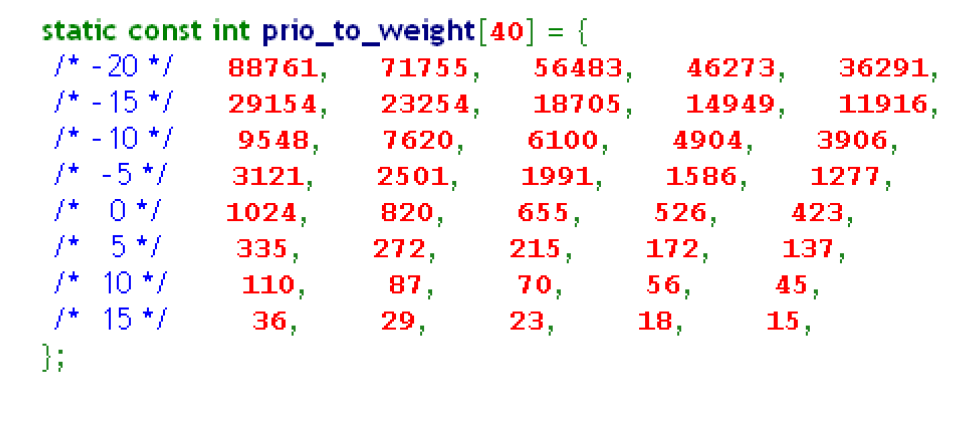
\includegraphics[width=10cm]{./figure/cfs_weight.png}
  \floatfoot{nice=0时,虚拟时间等于物理时间  }
  }
\end{figure}

所有虚拟时间挂在红黑树上,每次linux调度虚拟时间最小的进程运行。

\chapter{调整优先级}

~\\调度优先级是内核分配给进程的代表执行先后可能的整数(-20-19)
整数值越小,优先级越高。bash shell默认以优先级0来启动所有进程,可通过nice命令和renice调整。
\section{用 nice 改变进程优先级}
对于普通用户来说,只可以以更低优先级运行命令,更高优先级运行命令需要高级用户权限。
nice命令是为未运行命令指定运行时调度优先级的,如果是已运行的命令则需要renice命令
\begin{latexcmd}[label=nice命令改变进程优先级]
#以10优先级值后台运行httpd命令
nice -n 10 httpd &

-n后面整数指定httpd命令运行的优先级
httpd即要改变优先级的命令
&表示此命令为后台运行
\end{latexcmd}
\begin{tcolorbox}[colback=blue!5,colframe=blue!75!black,title=nice设置进程视频]
\videoattach{3- nice.avi}{nice设置进程.avi}{https://share.weiyun.com/50Ij0ba}
\end{tcolorbox}

\section{用 renice 改变进程优先级}

renice命令与nice命令用法一样,限制也一样(普通用户只能以更低的调度优先级运行命令),惟一不同就是可以更新正在运行命令的调度优先级。
\begin{table}[!htbp]
\stabbox{2.2cm}
{\caption{Linux renice 命令参数含义}\label{}}
{\begin{tabular*}{\cflwidth}{@{\hspace{5pt}}@{\extracolsep{\fill}}*{3}{@{\hspace{-3pt}}l}}
    \heiti{参数} &  \heiti{含义 }              \\
    %\toprule
    -g &  使用程序群组名称,修改所有隶属于该程序群组的程序的优先权。             \\
    -p &   改变该程序的优先权等级,此参数为预设值。          \\
    -u &  指定用户名称,修改所有隶属于该用户的程序的优先权。      \\
\end{tabular*}
\floatfoot*{}
}
\end{table}

\begin{latexcmd}[label=nice命令改变进程优先级]
#PID为5200的进程nice设为-5
renice -5 -p 5200
\end{latexcmd}
\begin{tcolorbox}[colback=blue!5,colframe=blue!75!black,title=renice设置进程视频]
\videoattach{2- renice.avi}{renice设置进程.avi}{https://share.weiyun.com/5kRR0lo}
\end{tcolorbox}

\section{用 chrt 改变进程优先级}
使用实时调度策略,必须具有root权限。
chrt 命令的策略选项
\begin{table}[!htbp]
\stabbox{3.0cm}
{\caption{Linux chrt 命令参数含义}\label{}}
{\begin{tabular*}{\cflwidth}{@{\hspace{5pt}}@{\extracolsep{\fill}}*{4}{@{\hspace{-3pt}}l}}
    \heiti{短选项} & \heiti{长选项 }  & \heiti{詳細 }              \\
    %\toprule
    -f & --fifo   &  调度器设成 SCHED\_FIFO              \\
    -o & --other  &   调度器设成 SCHED\_OTHER            \\
    -r & --rr     &   调度器设成 SCHED\_RR           \\
    -a & --all-tasks &  设置Pid号对应的所有线程              \\
\end{tabular*}
\floatfoot*{}
}
\end{table}

\begin{latexcmd}[label=chrt使用方法]
# 确认某个进程的属性可以通过指定 -p 或 --pid 并指定进程ID,用法如下:
# chrt -p 468
pid 468's current scheduling policy: SCHED_FIFO
pid 468's current scheduling priority: 85

# chrt -p 476
pid 476's current scheduling policy: SCHED_OTHER
pid 476's current scheduling priority: 0

# 将PID 1000 的进程设定成 SCHED_FIFO,优先级设定成50。
chrt -f -p 50 1000

# 将PID 1000 的进程设定成 SCHED_OTHER,优先级设定成0。
chrt -o -p 0 1000

# 起动 /bin/my-app 设定成 SCHED_FIFO,优先级设定成36。
chrt -f 36 /bin/my-app
\end{latexcmd}
\begin{tcolorbox}[colback=blue!5,colframe=blue!75!black,title=chrt设置进程视频]
\videoattach{4- chrt.avi}{chrt设置进程.avi}{https://share.weiyun.com/5c3Upbl}
\end{tcolorbox}


%%% Local Variables:
%%% TeX-master: "main"
%%% End:
